% !TEX program = xelatex
% !TEX encoding = UTF-8

% ---------------------------------------------------------------------------- %
% Document configuration
% ---------------------------------------------------------------------------- %

\documentclass[a4paper]{report}

% Margins
\usepackage[
top    = 2.75cm,
bottom = 2.75cm,
left   = 2.00cm,
right  = 2.00cm]{geometry}

% Paragraph indent
\setlength{\parindent}{15pt}

% Line height
\usepackage{setspace}
\onehalfspacing

% Font face
\usepackage{fontspec}
\setmainfont{Helvetica}
\setsansfont{Helvetica}
\setmonofont{Menlo}

% Multiple columns
\usepackage{multicol}

% ---------------------------------------------------------------------------- %
% Language configuration
% ---------------------------------------------------------------------------- %

\usepackage[danish]{babel}

\usepackage{csquotes}
\usepackage[nottoc]{tocbibind}

\usepackage[obeyspaces]{url}
\usepackage{hyperref}

% ---------------------------------------------------------------------------- %
% Header/footer configuration
% ---------------------------------------------------------------------------- %

\usepackage{fancyhdr}
\pagestyle{fancy}

% ---------------------------------------------------------------------------- %
% Graphics configuration
% ---------------------------------------------------------------------------- %

\usepackage{graphicx}
\usepackage{wrapfig}
\graphicspath{{images/}}

% ---------------------------------------------------------------------------- %
% Code highlighting
% ---------------------------------------------------------------------------- %

\usepackage{minted}

% Highlight theme
\usemintedstyle{trac}

% ---------------------------------------------------------------------------- %
% List configuration
% ---------------------------------------------------------------------------- %

\let\oldenumerate\enumerate
\renewcommand{\enumerate}{
  \oldenumerate
  \setlength{\itemsep}{1pt}
  \setlength{\parskip}{0pt}
  \setlength{\parsep}{0pt}
}

\let\olditemize\itemize
\renewcommand{\itemize}{
  \olditemize
  \setlength{\itemsep}{1pt}
  \setlength{\parskip}{0pt}
  \setlength{\parsep}{0pt}
}

% ---------------------------------------------------------------------------- %
% Bibliography configuration
% ---------------------------------------------------------------------------- %

\usepackage[
  backend=biber,
  style=authoryear
]{biblatex}
\bibliography{bibliography}

% ---------------------------------------------------------------------------- %
% Appendice configuration
% ---------------------------------------------------------------------------- %

\usepackage[titletoc]{appendix}
\usepackage{pdfpages}

% ---------------------------------------------------------------------------- %

\begin{document}

% ---------------------------------------------------------------------------- %
% Title page
% ---------------------------------------------------------------------------- %

% ---------------------------------------------------------------------------- %
% Title page
% ---------------------------------------------------------------------------- %

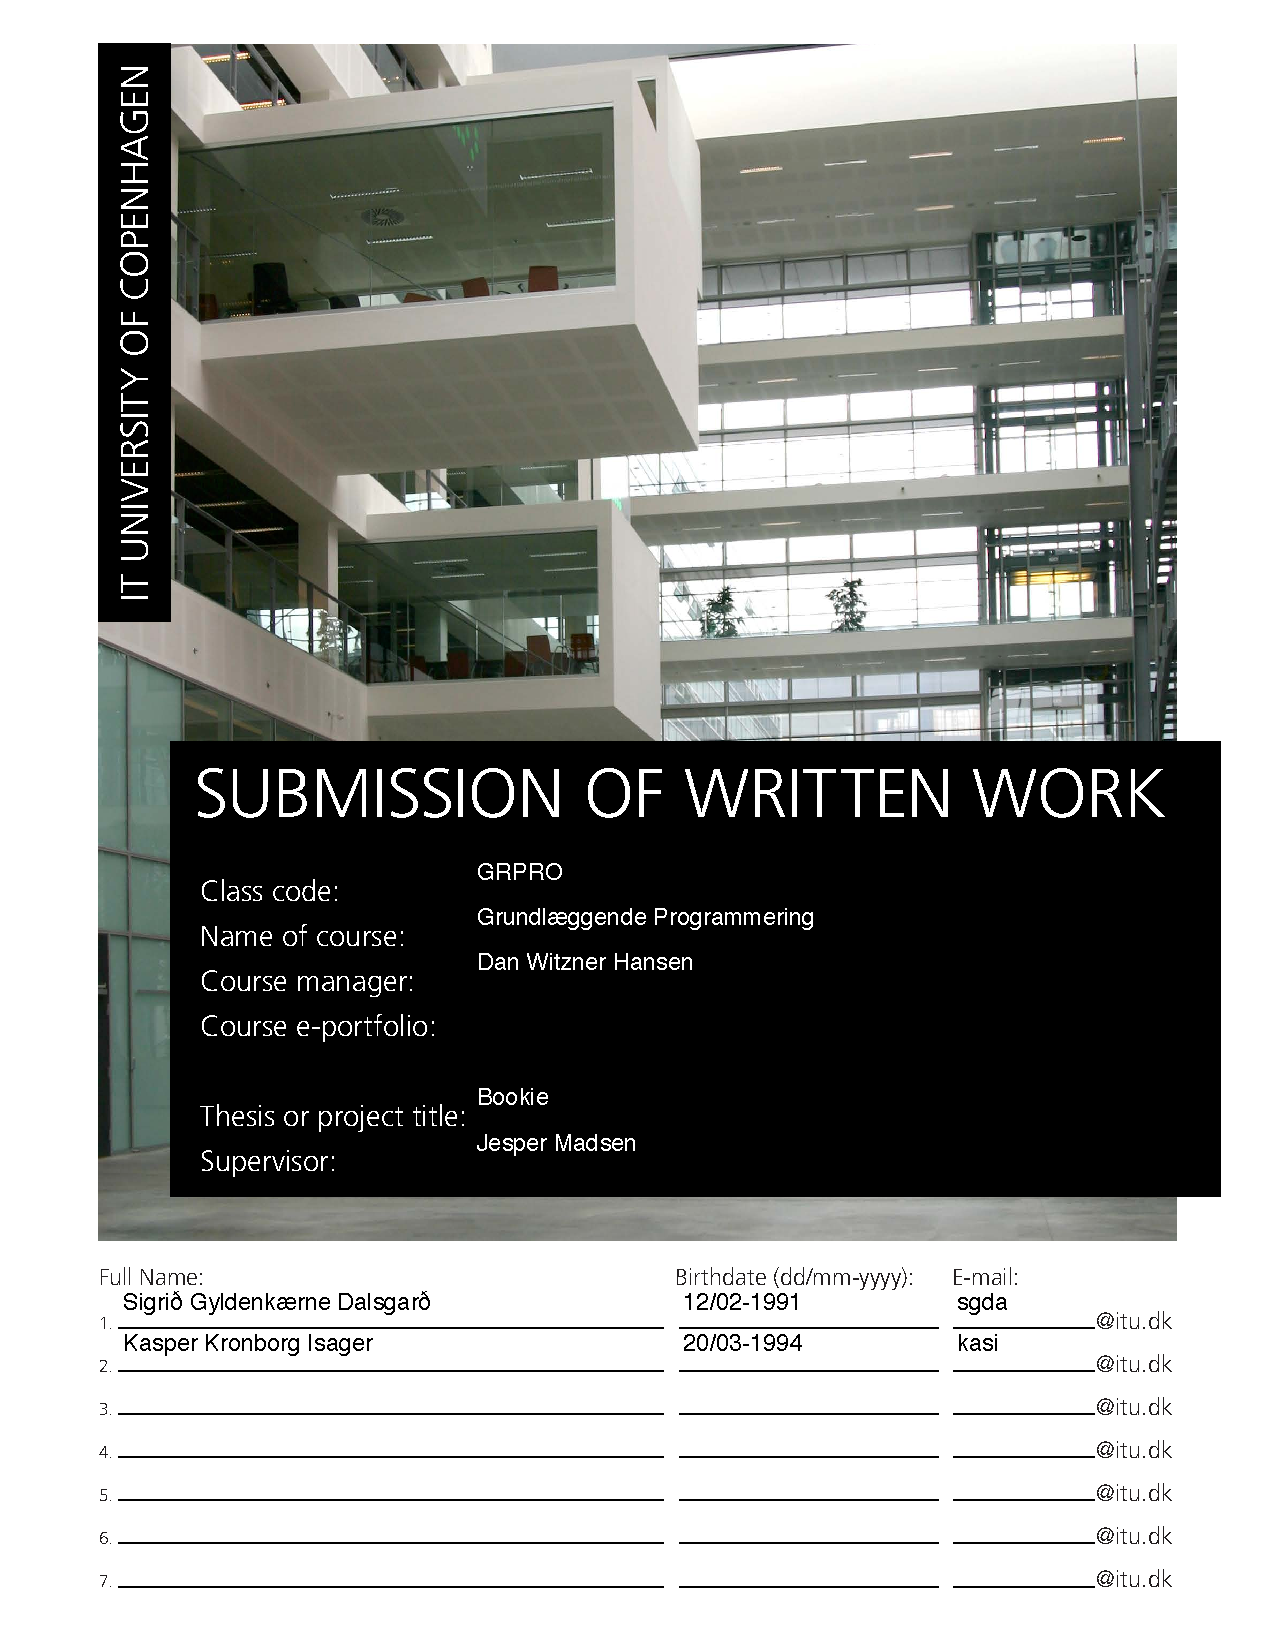
\includepdf{cover.pdf}

\begin{titlepage}

\center

\LARGE{IT-Universitetet i København}\\[1.5cm]
\Large{Grundlæggende Programmering}\\[0.5cm]
\large{Eksamensprojekt}

\vfill

\huge{\bfseries Bookie}

\vfill

\begin{minipage}[t]{0.4\textwidth}
\begin{flushleft} \large
  \emph{Forfattere:}\\
  Sigrid Gyldenkærne Dalsgard \\
  Kasper Kronborg Isager
\end{flushleft}
\end{minipage}
\begin{minipage}[t]{0.4\textwidth}
\begin{flushright} \large
  \emph{Vejleder:} \\
  Jesper Wendel Madsen
\end{flushright}
\end{minipage}

\vfill

\large{17. december 2014}

\end{titlepage}


% ---------------------------------------------------------------------------- %
% Abstract
% ---------------------------------------------------------------------------- %

% ---------------------------------------------------------------------------- %
% Abstract
% ---------------------------------------------------------------------------- %

\begin{abstract}
\end{abstract}


% ---------------------------------------------------------------------------- %
% Table of contents
% ---------------------------------------------------------------------------- %

\tableofcontents

% ---------------------------------------------------------------------------- %
% Chapters
% ---------------------------------------------------------------------------- %

\chapter{Forord}
\chapter{Baggrund og problemstilling}
\label{chapter:baggrund-og-problemstilling}

En ekspedient skal med et reservationssystem kunne betjene billetlugen og telefonen i en mindre biograf. Ekspedienten skal kunne reservere billetter til forestillinger samt lave ændringer på eller slette eksisterende reservationer. Al data håndteret af systemet skal gemmes i en relationsdatabase, således at reservationer ikke går tabt.

\section{Brugerhistorier}

Følgende brugerhistorier (\cite{wiki:user-story}) er udarbejdet som krav til reservationssystemet, og tager udgangspunkt i ekspedientens, såvel som kundens rolle i reservationsprocessen.

\subsection{Ekspedientens rolle}

\begin{itemize}
  \item Som en ekspedient vil jeg reservere en eller flere billetter til den forestilling, som en kunde måtte ønske.
  \item Som en ekspedient vil jeg sortere i forestillingerne, så jeg kan finde den forestilling, som en kunde måtte ønske.
  \item Som en ekspedient vil jeg se hvilke sæder er ledige til en given forestilling, så jeg kan finde de sæder, som en kunde måtte ønske.
  \item Som en ekspedient vil jeg knytte en kundes telefonnummer til en reservation, så jeg senere kan finde den igen.
  \item Som en ekspedient vil jeg søge på en kundes telefonnummer, så jeg kan finde deres reservationer igen.
  \item Som en ekspedient vil jeg slette en kundes reservation, hvis de ønsker det.
  \item Som en ekspedient vil jeg ændre en kundes reservation, hvis de ønsker det.
\end{itemize}
  
\subsection{Kundens rolle}

\begin{itemize}
  \item Som en kunde vil jeg se en bestemt eller vilkårlig film på en bestemt eller vilkårlig dag samt et bestemt eller vilkårligt tidspunkt af dagen.
  \item Som en kunde vil jeg have de ledige sæder, som jeg bedst synes om.
  \item Som en kunde vil jeg afreservere mine billetter hvis jeg ikke kan komme til forestillingen.
  \item Som en kunde vil jeg tilføje billetter til fra min reservation hvis nødvendigt.
  \item Som en kunde vil jeg fjerne billetter fra min reservation hvis nødvendigt.
\end{itemize}

Der er en chance for, at der ikke er nok billetter til den valgte forestilling, eller at der ikke er en forestilling på det valgte tidspunkt. Også har vi det eksempel, at hvis en kunde ringer og spørger efter 10 billetter til en bestemt forestilling, hvor der er pladser nok, men pladserne er desværre ikke placeret ved siden af hinanden, hvilke muligheder er der så? Disse problemer kan visuelt afkodes af brugergrænsefladen. Hvis biografen ikke kan udbyde kundens efterspørgsel, så vil der ikke ske andet, end at kunden må finde en anden forestilling eller acceptere, at han/hun ikke kommer i biograf på det valgte tidspunkt.

Brugerhistorierne bliver alle løst på forskellige måder. For det første må der eksistere nogle forestillinger, sale, rækker og sæder før der kan laves nogle reservationer. Forestillingerne i sig selv er en kombination af film, sal, tidspunkt og dag. Disse forskellige elementer skal kunne ses på brugergrænsefladen. Da rækkerne og sæderne skal kunne reserveres til kunder, må der ikke være muligt for ekspedienten at dobbeltreservere.

For det andet skal man bl.a. kunne koble et kunde-id (i form af telefonnummer) sammen med en forestilling, hvorefter disse informationer skal kunne gemmes, hentes igen, evt. redigeres og slettes. Databaser bliver her et nødvendigt redskab.

Der er taget det valg, at bruge et klient-tungt system, som inkluderer at det godt kan bruges uafhængigt af en server. Der er ikke et behov for forbindelse til hverken en server eller et netværk. Al data er placeret lokalt, og bl.a. fordi vi får givet, at biografen kun skal have én billetluge og tillader ikke reservationer over nettet. Dette inkluderer, at det ikke er muligt at lave forskellige opdateringer til databasen på samme tid.

Det færdige projekt skal kunne håndtere alle krav, som er blevet stillede. Det skal kunne tilfredsstille kunden og ekspedienten således, at der hverken er problemer eller mangel på muligheder vedrørende reservationer eller redigering af dem.

\chapter{Problemanalyse}
\label{chapter:problem}

\section{Databasedesign}

\subsection{Film}

\subsection{Sal}

\subsection{Forestilling}

\subsection{Billet}

\subsection{Reservation}

\section{Præsentation af data}

Det første skridt mod et program er ofte et mockup. Et mockup visualiserer en idé, og får en brainstorm til at være mere konkret. Ud fra dette bliver der arbejdet med hvert enkle element i mockup'en, hvilket ofte gør, at hvert element bliver en klasse i en kode. Ud fra mockup'en er det også lettere at se hvilke klasser skal være forbundet til hinanden, og derefter også hvor data skal placeres (hvis data skal være med).

\section{Beskrivelse}

Vi har valgt at bruge et program (ud af mange) der hedder Balsamiq Mockups.
Det står i problemformuleringen, at Bookie ikke skal være indviklet, hvilket bliver reducéret ti, at Bookie kun skal kunne det mest basale, som et reservationssystem kræver. Data er en nødvendighed, men der er forskellige måder at repræsentere den på.

Ud fra vores mockup, repræsenterer vi data på den måde, at der først bliver valgt en film (\ref{mockup: balsamiq-showtimes}), hvorefter man kommer ind på et vindue, hvor der er muligt at se hvilke dage og tidspunkter den valgte film bliver vist (\ref{mockup: balsamiq-showtimes1}). Inde på næste vindue bliver det så muligt at reservere pladser (\ref{mockup: balsamiq-auditorium}), hvilke så ender inde på \textit{Reservationer} (\ref{mockup: balsamiq-reservation}).

I forhold til vores mockup, er der på startsiden (\ref{mockup: balsamiq-showtimes}) lavet en liste som repræsenterer filmene som data. Til hver film er der en tabel (\ref{mockup: balsamiq-showtimes1}), hvor rækkerne beskriver tidspunkter på dagen, og kolonnerne dagene i ugen. Til hver forestilling er der en sal (\ref{mockup: balsamiq-auditorium}), hvor sæderne er delt op i et gitter, og hvor hvert sæde repræsenterer en billet. Hvilket inkluderer i, at en billet er forbundet med et tidspunkt og en sal, som er forbundet til en film. Dog har \textit{Reservationer} også en liste, men denne liste indeholder billetter. Det vil sige, at billetterne også er forbundet til \textit{Reservationer}, men ikke omvendt.

Inde på \textit{Reservationer} er der også muligt at søge efter en bestemt reservation ved at skrive et telefonnummer ind på \textit{søg}-feltet. Dette felt vil så filtrere numrene i tabellen.

Idéen fungerer fint, men JavaFX har ikke samarbejdet på et optimalt plan, hvilket har fået den endelige brugergrænseflade til at blive lidt anderledes, den har en lidt anden måde at repræsentere data på. Som det også kan ses i \textit{Brugervejledning og eksempel}, så er alle forestillinger i samme tabel, med salene til højre for tabellen. Igen er data fra reservationerne repræsenteret i et gitter. \textit{Reservationer} i Bookie minder meget om mockup'en. 

\subsection{Mockups}

\begin{figure}[h]
  \centering
  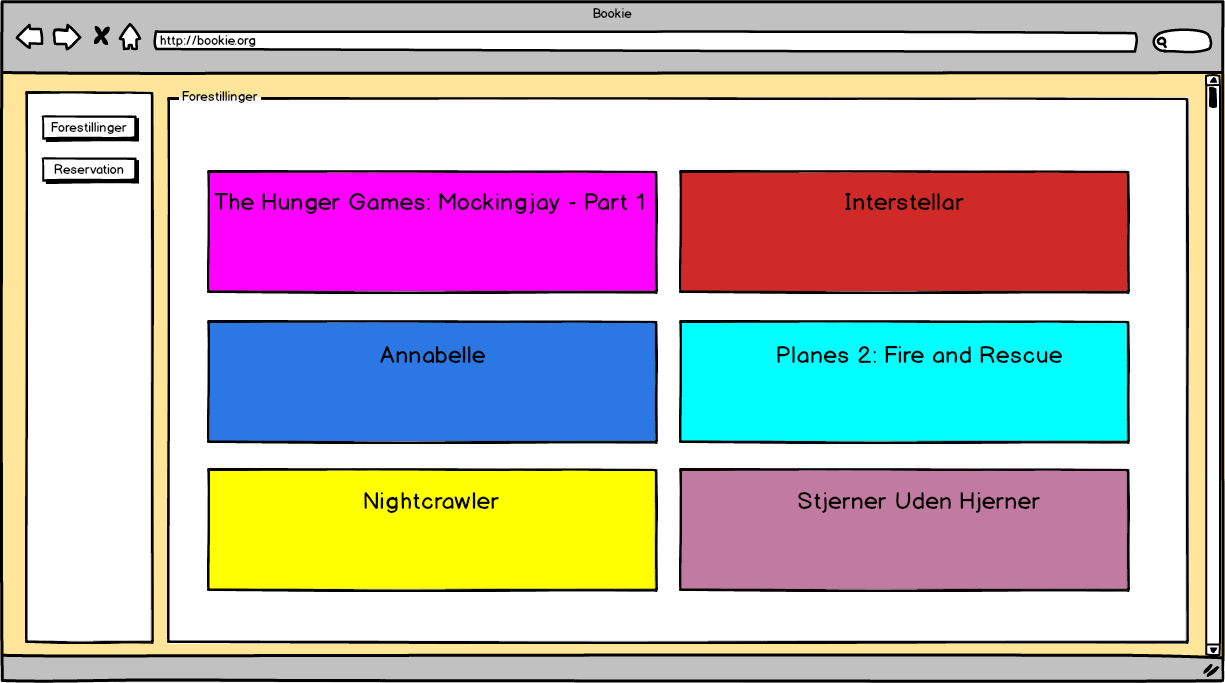
\includegraphics[width=\textwidth]{balsamiq-showtimes.png}
  \caption{Mockup - Bookie startside}
  \label{mockup: balsamiq-showtimes}
\end{figure}

\begin{figure}[h]
  \centering
  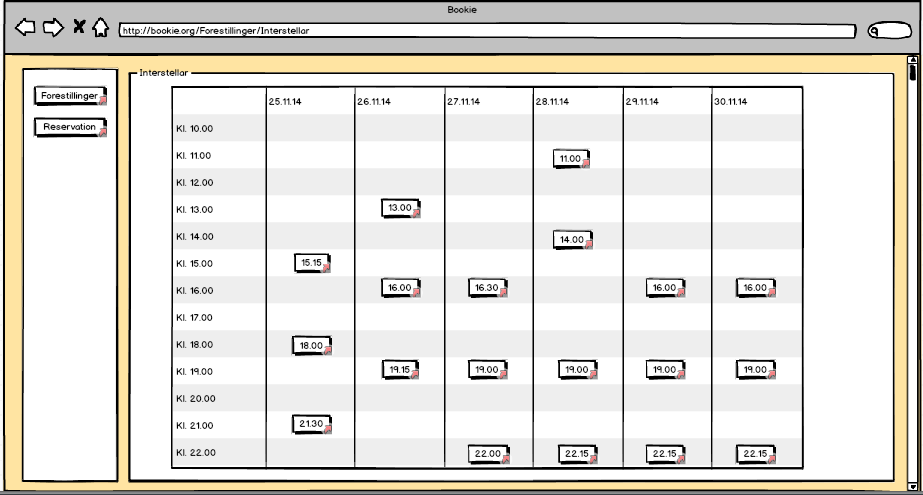
\includegraphics[width=\textwidth]{balsamiq-showtimes1.png}
  \caption{Mockup - tidspunkter}
  \label{mockup: balsamiq-showtimes1}
\end{figure}

\begin{figure}[h]
  \centering
  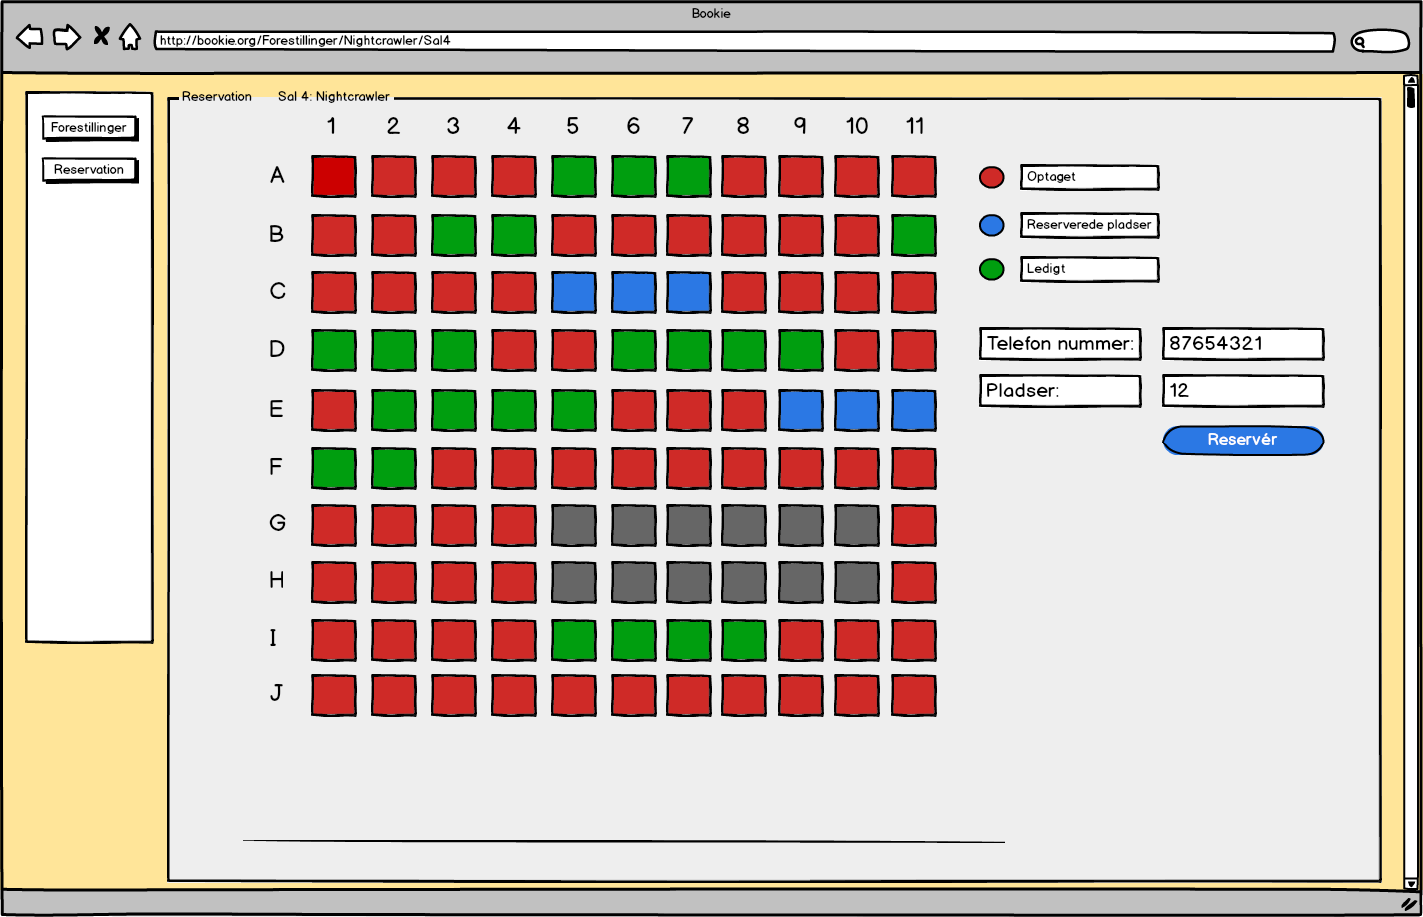
\includegraphics[width=\textwidth]{balsamiq-auditorium.png}
  \caption{Mockup - Eksempel på en sal}
  \label{mockup: balsamiq-auditorium}
\end{figure}

\begin{figure}[h]
  \centering
  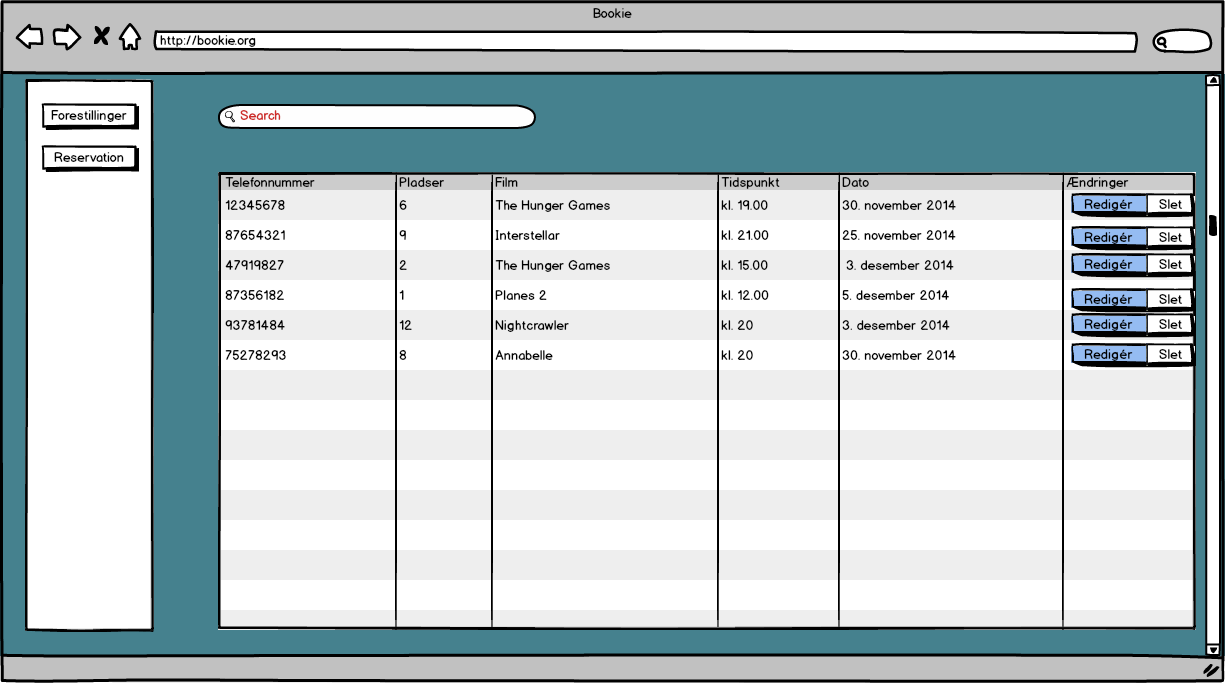
\includegraphics[width=\textwidth]{balsamiq-reservation.png}
  \caption{Mockup - Reservationer}
  \label{mockup: balsamiq-reservation}
\end{figure}

\section{Diskussion}

\section{Systemarkitektur}

Med udgangspunkt i de tidligere beskrevne krav til reservationssystemet, ser vi god grund til at benytte os af den ofte brugte \textit{Model-view-controller} arkitektur (forkortet \textit{MVC}). Denne beskriver en streng opdeling af et systems komponenter (\cite{wiki:mvc}):

\begin{itemize}
  \item
    \textbf{Model}
  
    En Model beskriver i MVC et stykke data samt den underliggende logik for dette. Dette oversættes i reservationssystemet til de forskellige typer af data, som skal håndteres: Film, reservationer, billetter, mv.
  \item
    \textbf{View}
    
    Et View beskriver i MVC præsentationen af et systems forskellige Models. I reservationssystemet oversættes dette til de FXML-filer, som benyttes til af opbygge den visuelle del af brugergrænsefladen og dermed præsentationen af systemets data.
  \item
    \textbf{Controller}
    
    En Controller er i MVC som oftest bindeledet mellem et View og dennes bagvedliggende Model og står for at håndterede brugerinput samt at supplere Views med deres tilhørende Models. Controllere i MVC er også set brugt udelukkende som fortolker af brugerinput, og deres forhold til Models og Views er derfor ikke nødvendigvis fastdefineret (\cite{burbeck1987}).
    
    Controllere i reservationssystemet er dermed de klasser, som i systemets FXML Views måtte være refererede via \texttt{fx:controller}-attributten.
\end{itemize}

\chapter{Brugervejledning}

I dette kapitel gennemgåes brugen af det udviklede reservationssystem, Bookie. Vejledningen vil undervejs blive understøttet af billeder, der har til formål af eksemplificere de tilhørende instruktioner.

\section{Forestillinger}

Når Bookie åbnes, vises fanen \textit{Forestillinger}, der indeholder listen af forestillinger samt reservationsskærmen som set på figur \ref{screenshot:bookie}. På denne figur ses ydermere følgende elementer: Placeringen af lærredet i biografsalen, legenden over sædestatus (ledig, valgt, reserveret, og købt), samt formularen til reservation af sæder. En biografsal er imidlertid endnu ikke synlig, da der ikke er valgt en forestilling.

\begin{figure}[h]
  \centering
  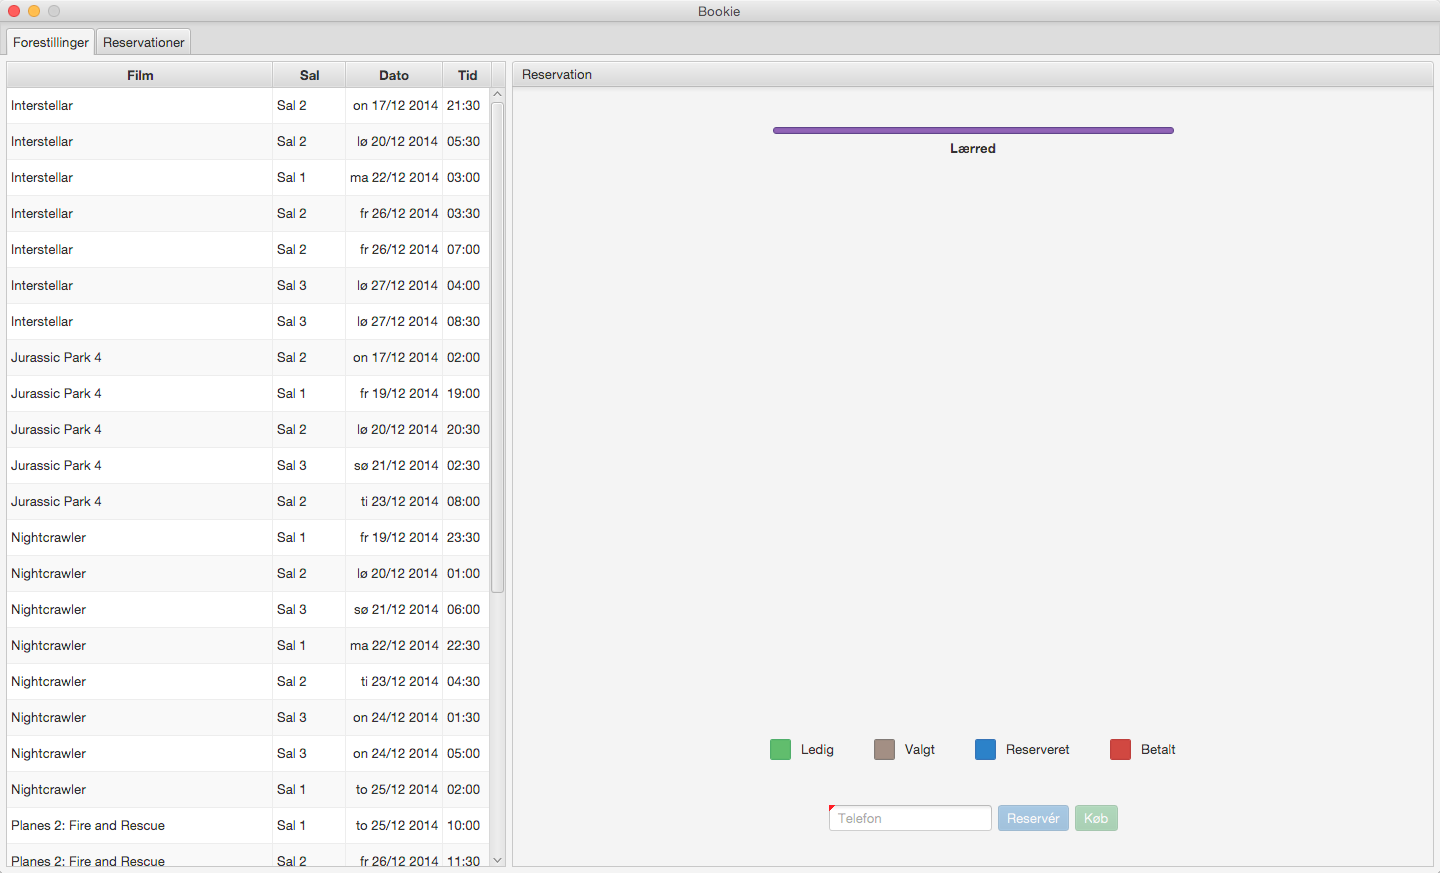
\includegraphics[width=\textwidth]{showtimes.png}
  \caption{Bookies startside straks efter opstart}
  \label{screenshot:bookie}
\end{figure}

\subsection{Valg af forestilling}

Der er mulighed for at sortere listen af forestillinger efter film, sal, dato, og tidspunkt. Det er derfor let at finde præcist den forestilling, som kunden måtte ønske. En forestilling vælges ved at klikke på den i listen.

\begin{figure}[h]
  \centering
  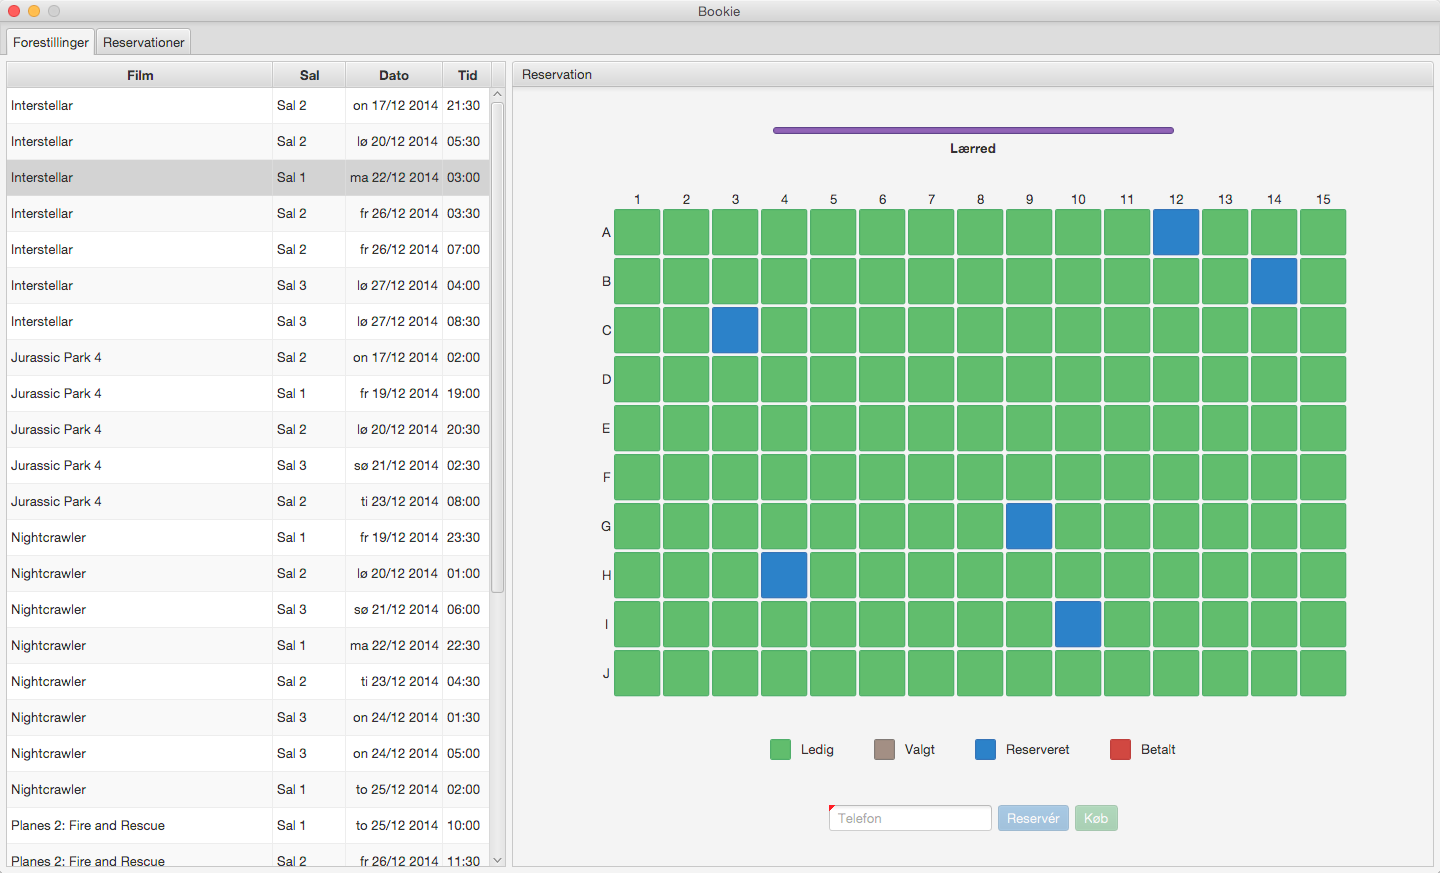
\includegraphics[width=\textwidth]{chosen-showtime.png}
  \caption{Udseende af biografsalen efter valg af forestilling}
  \label{screenshot:chosen-showtime}
\end{figure}

\subsection{Valg af sæder}

\begin{wrapfigure}[4]{r}{0.4\textwidth}
  \centering
  \vspace{-12pt}
  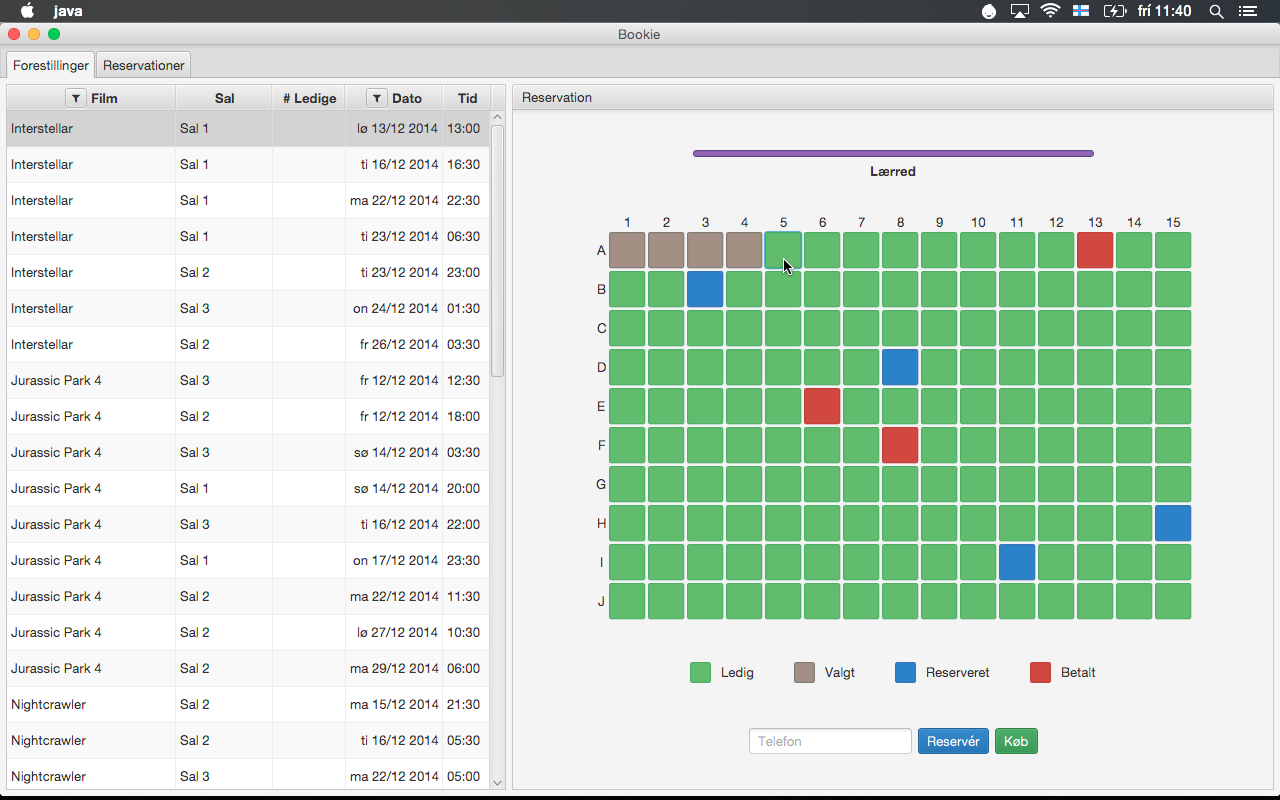
\includegraphics[width=0.35\textwidth]{chosen-seats.png}
  \caption{Eksempel på valg af sæder}
  \label{screenshot:chosen-seats}
\end{wrapfigure}

Holdes musen hen over et af de ledige sæder (markerede med grøn) og trykkes der på det, vil sædet skifte farve til grå som indikation på, at det er valgt til reservation.

Det er ikke muligt at oprette en reservation uden minimum at vælge et enkelt sæde.

\subsection{Reservation af sæder}

Efter de ønskede sæder er blevet valgt, er det muligt at indtaste et telefonnummer (se figur \ref{screenshot:phone-number}) for reservationen. Trykkes der derefter på \textit{Reservér}-knappen, ændres sædernes farve til blå som indikation på, at reservationen er gennemført. Det samme gør gældende med \textit{Køb-knappen}, hvor sædernes farve dog istedet vil ændres til rød. Efter gennemført reservation vil telefonnummer-feltet blive ryddet.

\begin{figure}[h]
  \centering
  \begin{minipage}[b]{0.4\linewidth}
    \centering
    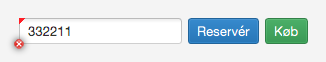
\includegraphics[width=\textwidth]{phone-number-invalid.png}
  \end{minipage}
  \hspace{0.5cm}
  \begin{minipage}[b]{0.4\linewidth}
    \centering
    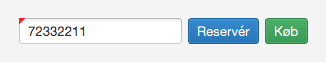
\includegraphics[width=\textwidth]{phone-number.png}
  \end{minipage}

  \caption{Eksempel på indtastning af ugyldigt (tv.) og gyldigt (th.) telefonnummer}
  \label{screenshot:phone-number}
\end{figure}

\section{Reservationer}

Når en reservation er oprettet, kan denne findes under fanen \textit{Reservationer}. Alle eksisterende reservationer kan ligeledes findes under denne fane som set på figur \ref{screenshot:all-reservations}.

\begin{figure}[h]
  \centering
  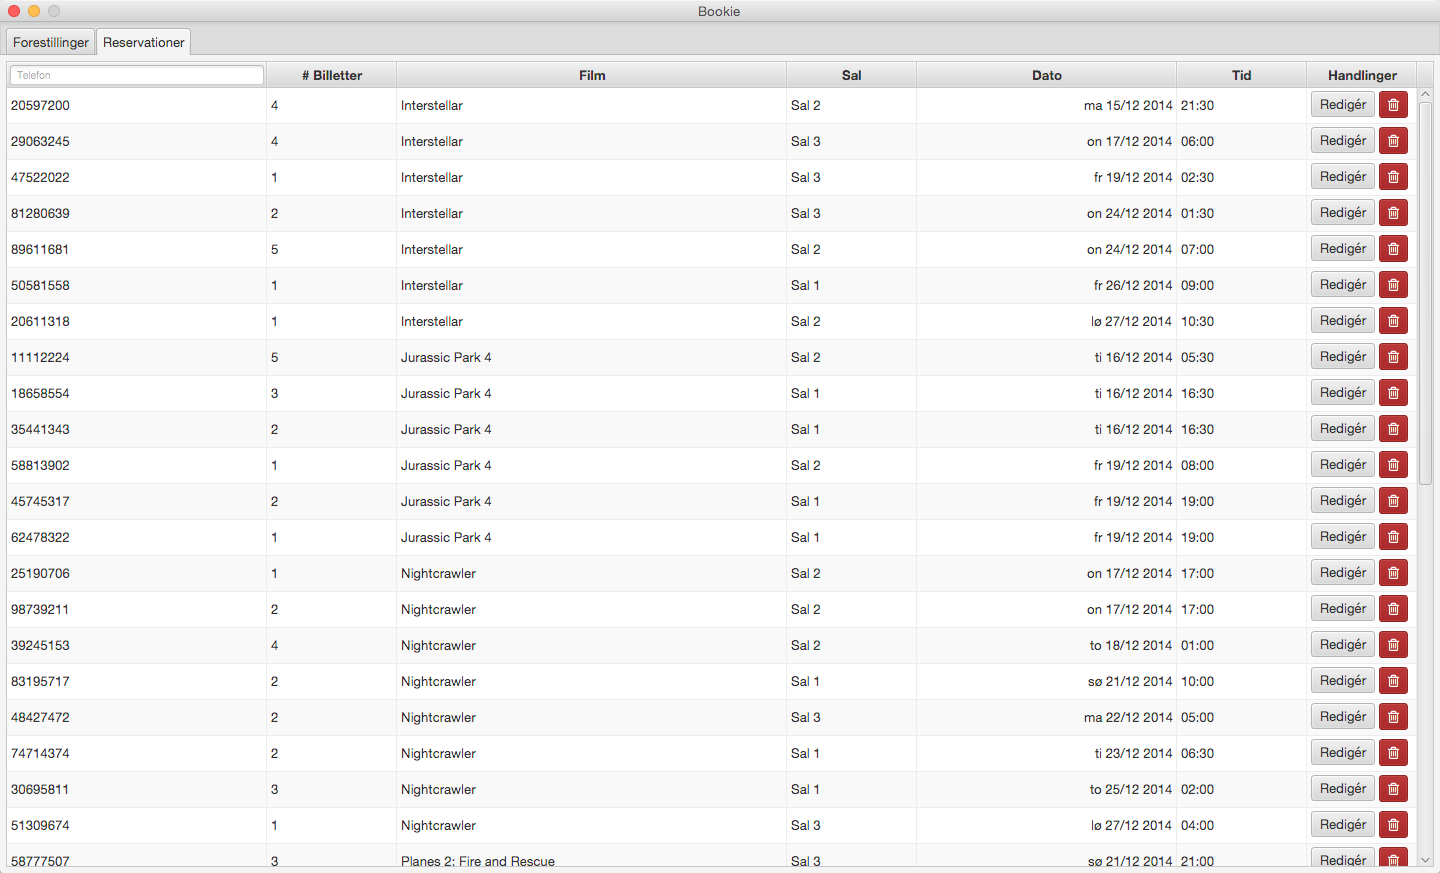
\includegraphics[width=\textwidth]{reservations.png}
  \caption{Visning af alle reservationer}
  \label{screenshot:all-reservations}
\end{figure}

\subsection{Filtrering af telefonnumre}

\begin{wrapfigure}[3]{r}{0.4\textwidth}
  \centering
  \vspace{-12pt}
  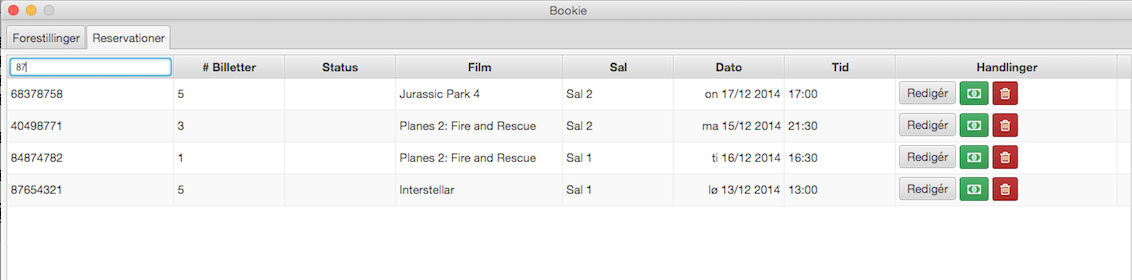
\includegraphics[width=0.35\textwidth]{filter3.png}
  \caption{Filtrering af telefonnumre}
  \label{screenshot:filter3}
\end{wrapfigure}

I øverste, venstre hjørne af reservationslisten findes et felt til filtrering af telefonnumrene (figur \ref{screenshot:filter3}). Der kan søges på enten fulde telefonnumre eller brydstykker af disse, hvilket gør det let af finde den eller de ønskede reservationer.

\subsection{Redigering af reservationer}

\begin{wrapfigure}{r}{0.4\textwidth}
  \centering
  \vspace{-12pt}
  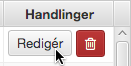
\includegraphics[width=0.2\textwidth]{edit-button.png}
  \caption{Mulighed for redigering af reservationer}
  \label{screenshot:edit-button}
\end{wrapfigure}

Når den ønskede reservation er fundet, kan denne hurtigt redigeres ved at trykke på \textit{Redigér}-knappen fundet i højre side af skærmen (figur \ref{screenshot:edit-button}). \textit{Forestillinger}-fanen vil da blive vist, hvorefter der enten kan fjernes sæder fra eller føjes flere sæder til den pågældende reservation (figur \ref{screenshot:edit-button}).

Skulle det ske, at reservationen ønskes flyttet til en anden forestilling, skal reservationen da først slettes, hvorefter en ny reservation kan oprettes til den ønskede forestilling. Sletning af reservationer gennemgåes nedenfor.

\subsection{Sletning af reservationer}

\begin{wrapfigure}{r}{0.4\textwidth}
  \centering
  \vspace{-12pt}
  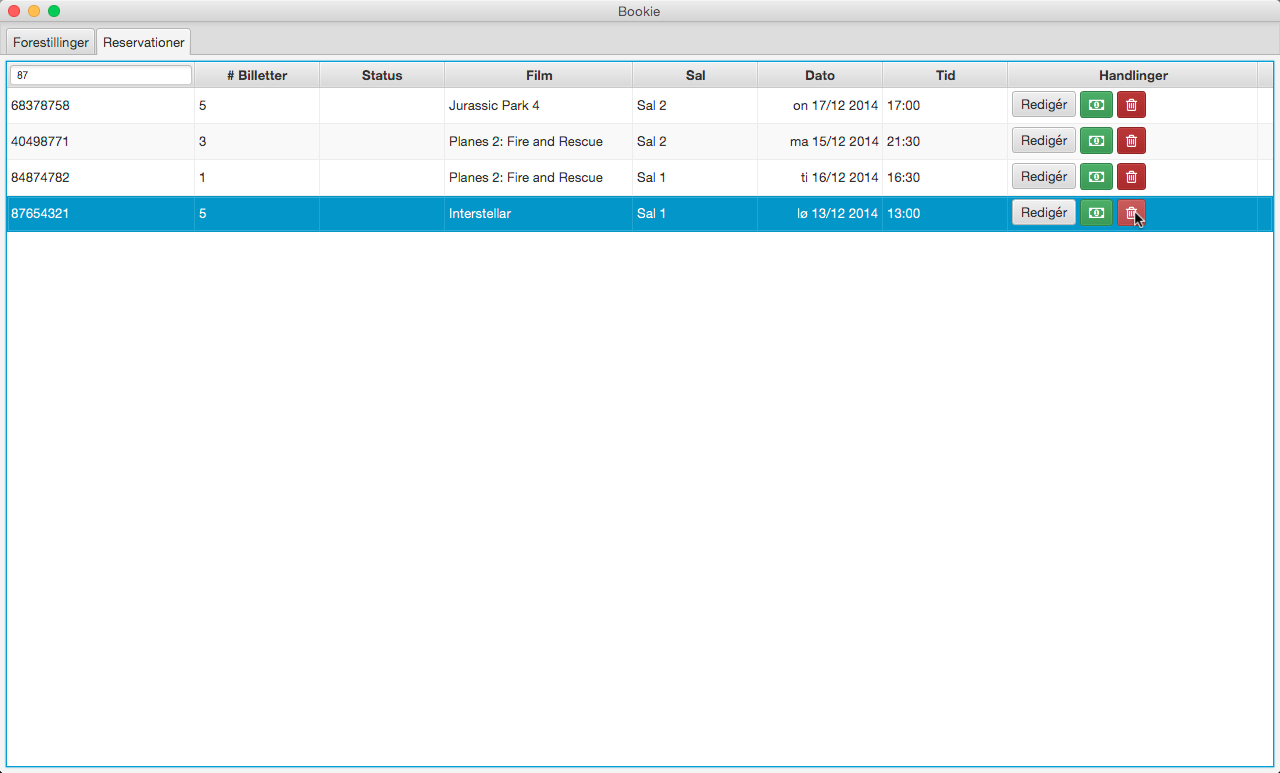
\includegraphics[width=0.2\textwidth]{delete-button.png}
  \caption{Mulighed for sletning af reservationer}
  \label{screenshot:delete-button}
\end{wrapfigure}

At slette er reservation er lige så smertefrit som at arbejde i resten af Bookie. Bliver der trykket på den røde knap med skraldespand-ikonet ved siden af \textit{Redigér}-knappen (som ses på \ref{screenshot:delete-button}, så kommer et pop-up (figur \ref{screenshot:delete-reservation}, hvor man kan vælge mellem \textit{cancel} eller \textit{ok}. Vælger ekspedienten \textit{cancel}, sker der ikke noget andet end, at pop-up'et forsvinder og \textit{Reservationer} forbliver som før. Vælger ekspedienten \textit{ok}, forsvinder den valgte reservation fra listen.

\begin{figure} [h]
  \centering
  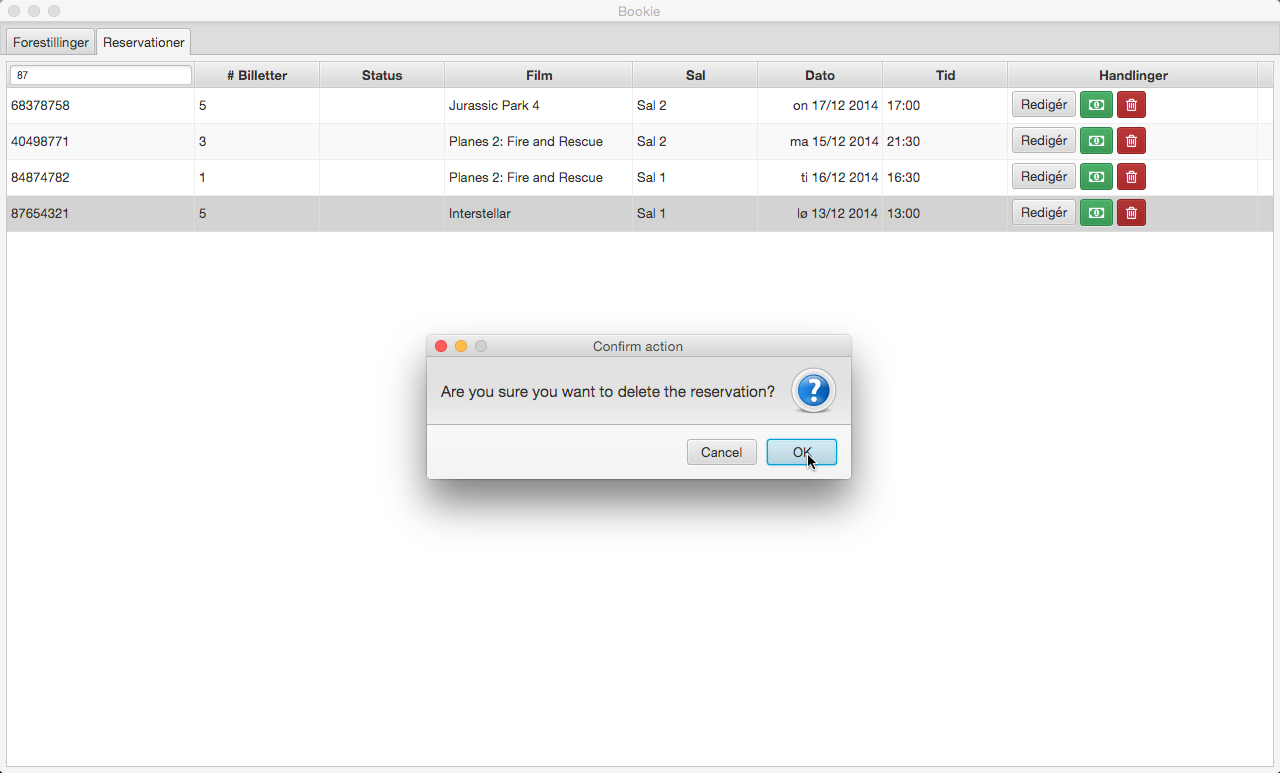
\includegraphics[width=0.4\textwidth]{delete-reservation.png}
  \caption{Sletning af reservation.}
  \label{screenshot:delete-reservation}
\end{figure}
\chapter{Teknisk beskrivelse}

\begin{wrapfigure}{r}{0.5\textwidth}
  \centering
  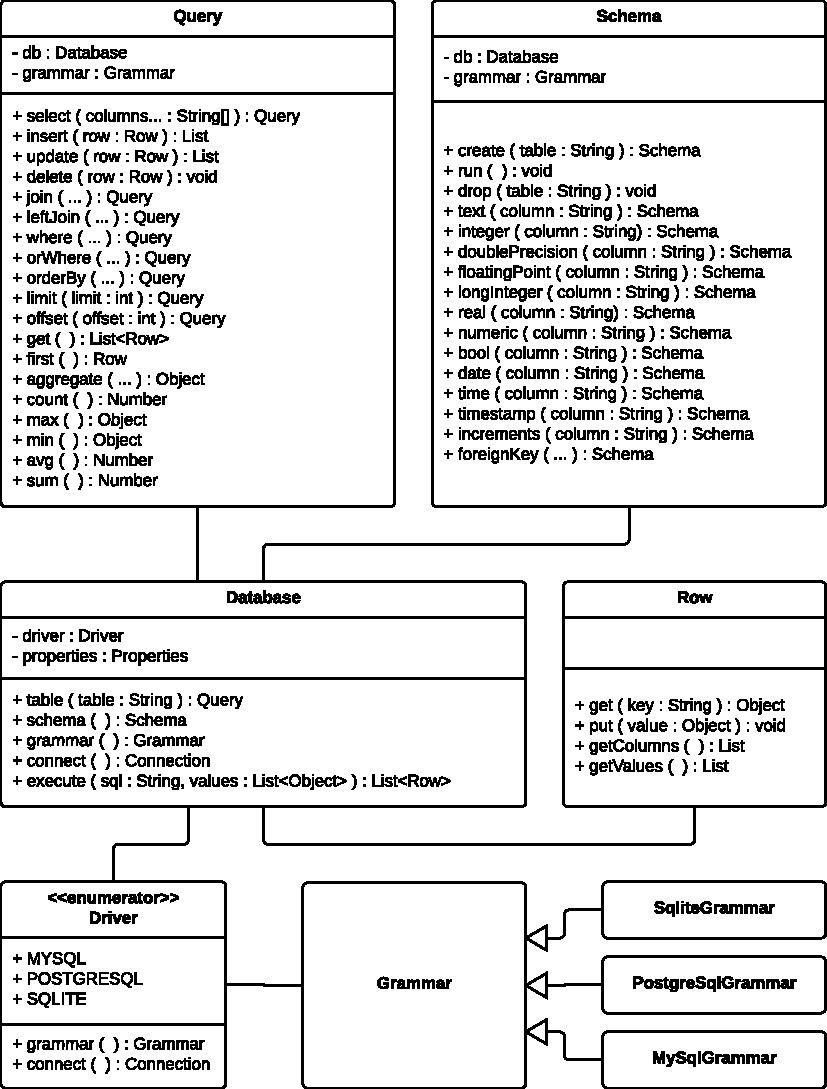
\includegraphics[scale=0.75]{images/database-abstraction.pdf}
  \caption{Klassediagram over Donkeys databaseabstraktion.}
\end{wrapfigure}

\chapter{Afprøvning}
\label{chapter:afproevning}

\section{Automatiserede tests}

I kraft af separationen mellem datamodeller og præsentationen samt håndteringen af disse, har vi valgt at implementere en række automatiserede tests udelukkende af datamodellerne.

Der er i samtlige tests, som involverer interaktion med en database, testet direkte mod de af Donkey understøttede databasesystemer. For at undgå utilsigtet indflydelse af tilstanden af testtabellerne, bliver disse derfor enten slettede eller tømt førend hver test. Ønskes testene kørt lokalt, gør vi derfor også opmærksomme på, at fungerende installationer af MySQL samt PostgreSQL er et krav. Disse skal ydermere være opsat med følgende databaser og tilhørende brugere (sans kodeord):

\begin{itemize}
  \item MySQL: \textbf{Database}: test, \textbf{bruger}: travis
  \item PostgreSQL: \textbf{Database}: test, \textbf{bruger}: postgres
\end{itemize}

\subsection{Kodedækning}
\label{subsection:kodedeakning}

\textit{Code coverage}-rapporter er blevet benyttede til at sikre en systematisk tilgang til implementation af tests. Disse rapporter er generede via kodedækningsredskabet JaCoCo\footnote{\url{https://github.com/jacoco/jacoco}} (se figur \ref{code-coverage:donkey}) og giver overblik over præcist hvilke instruktioner og eksekveringsgrene, der er berørte af de underliggende tests (\cite{wiki:code-cov}).

\begin{figure}[h]
\begin{minipage}[b]{0.45\linewidth}
  \centering
  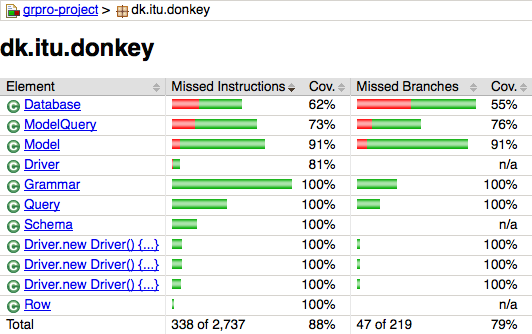
\includegraphics[width=\textwidth]{jacoco-donkey.png}
\end{minipage}
\hspace{0.5cm}
\begin{minipage}[b]{0.45\linewidth}
  \centering
  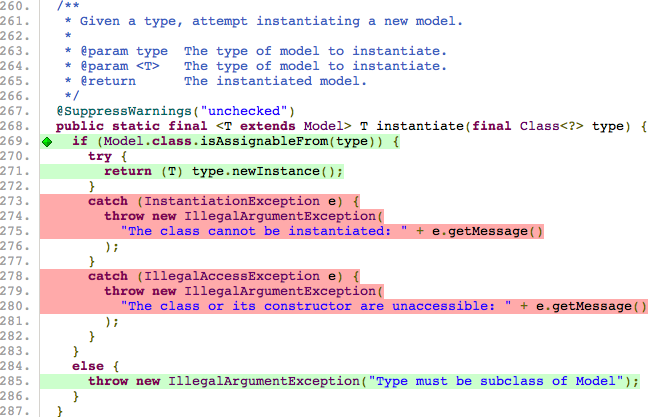
\includegraphics[width=\textwidth]{jacoco-model.png}
\end{minipage}
\caption{To udsnit af en JaCoCo kodedækningsrapport}
\label{code-coverage:donkey}
\end{figure}

Vi har tilstræbet en dækningsprocent på minimum 80\% gennem vores testning af databaseabstraktionen under antagelse af, at de sidste 20\% overvejende er ikke- eller svært-testbar kode.

Da kodedækningsrapporten er et sæt af genererede HTML-sider, er disse ikke medtagede som bilag, men kan istedet frit tilgåes via følgende webadresse: \url{http://kasperisager.github.io/bookie/coverage}.

Det bør nævnes, at kodedækningsrapporter ikke nødvendigvis er en fuldstændig vandtæt løsning, da de udelukkende kan udtale sig om den tilsigtede eksekvering af den kode, som måtte være under test. En metode kan derfor i dækningsrapporten fremgå som værende fuldt dækket uden nødvendigvis at fungere under alle tænkelige forhold.

\subsection{Analyse af resultat}

Samtlige klasser i databaseabstraktionen er som nævnt ovenfor forsøgt minimum 80\% dækkede med tests. En oversigt over de forskellige tests kan findes på adressen \url{http://kasperisager.github.io/bookie/tests}, mens testene i deres fulde format kan findes i bilag \ref{appendix:tests}.

Med udgangspunkt i kodedækningsrapporten kan vi med stor sikkerhed konkludere, at vores databaseabstraktion virker efter hensigten under de forhold, som den er blevet benyttet i reservationssystemet.

\section{Brugerafprøvning}

Mens systematisk automatiseret testning af reservationssystemets JavaFX-baserede brugergrænseflade endnu er en mangelvare, vil vi lade brugervejledningen stå som manuel brugerafprøvning. Den beskrevne funktionalitet i vejledningen er dermed den tilsigtede måde hvorpå reservationsystemets brugergrænseflade fungerer.
\chapter{Arbejdsproces}

\section{Brug af redskaber}

Der har under hele arbejdsforløbet været fokus på brug af redskaber, som kan afhjælpe ofte opstående problemstillinger i softwareprojekter:

\begin{itemize}
  \item Manglende versionskontrol af kode
  \item Oversete fejl ved introduktion af ny kode
  \item Manglende overblik ved testning af kode
  \item Manglende dokumentation af kode
  \item Inkonsistent struktur og udseende af kode
\end{itemize}

\subsection{Versionskontrol}

Al kode holdes under versionstyring ved hjælp af git\footnote{\url{http://www.git-scm.com/}}, hvilket sikrer, at alle udviklere på projektet har adgang til samme kodebase og inkrementalt kan indføre og holde styr på ændringer til denne. Som centraliseret git-server har vi benyttet os af GitHub\footnote{\url{https://github.com/}} og dennes udbud af gratis hosting af open source projekter: \url{https://github.com/kasperisager/bookie}

\subsection{Automatiseret testning}

For at komme problemet med oversete fejl ved introduktion af ny kode til livs, har vi valgt at benytte os af \textit{continuous integration} (forkortet \textit{CI}) i forlængelse af vores brug af versionskontrol. CI involverer løbende sammenfletning af de forskellige udvikleres arbejdskopier af kodebasen i sammenkobling med automatisk kørsel af tests ved hver sammenfletning (\cite{wiki:ci}). Dette sikrer, at fejl resulterende fra ikke-passerende tests kan findes førend de indtræder i andre udvikleres kopi af kodebasen.

Til afvikling af CI, og dermed automatisk kørsel af tests, har vi benyttet os af Travis CI\footnote{\url{https://travis-ci.org/}}, der ligesom GitHub tilbyder gratis service for open source projekter. Bookie kan findes på Travis CI via følgende adresse: \url{https://travis-ci.org/kasperisager/bookie}.

Som nævnt i kapitel \ref{subsection:kodedeakning} har vi med vores tests taget udgangspunkt i kodedækningsrapporter. For at opnå størst muligt overblik over dækningen af vores kode, har vi benyttet os af Coveralls\footnote{\url{https://coveralls.io}} til inkremental rapportering af kodebasens dækningsprocent som del af CI.
\chapter{Konklusion}




På grund af \textit{Donkey} er det en fornøjelse at arbejde med SQL. TEKST TEKST TEKST!! 
Programmet virker, dog kan der godt tilføjes nogle ændringer, for at få det til at virke optimalt. Nævner nogle af de ændringer, som ville være bedst for Bookie:

\begin{itemize}
  \item Det skal ikke være muligt at indtaste ugyldige telefonnumre, som f.eks. \textit{
  11222222} eller \textit{11400000}.
  %I dette tilfælde ville det være alarmcentralen og politiet, som det ville   gå ud over. Chancen for at nogen ville brokke sig, er rimelig stor. Hvilket ikke havde været så godt.
  \item At se hvor mange ledige pladser der er tilbage, ville være en stor hjælp for ekspedienten.
  \item Mulighed for at vælge sæder mere effektivt.
  % F.eks. at indtaste det antal af sæder man vil reservere, hvorefter det antal af sæder ville blive markeret, og man derefter ville kunne vælge hvilken placering de skulle have.
  
  \item Tastaturunderstøttelse. I tabellerne er det muligt at navigere med piletasterne, da dette kommer automatisk med JavaFX, men f.eks. at vælge sæder med pilene er indtil videre ikke muligt.
  
\end{itemize}
Et system kan altid arbejdes videre på, men på et tidspunkt bliver man nødt til at sige stop.



Alt i alt klarer Bookie opgaven godt.

% ---------------------------------------------------------------------------- %
% Bibliography
% ---------------------------------------------------------------------------- %

% Include all citations by default.
\nocite{*}

\printbibliography[heading=bibintoc]

% ---------------------------------------------------------------------------- %
% Figures and tables
% ---------------------------------------------------------------------------- %

\listoffigures
\listoftables

% ---------------------------------------------------------------------------- %
% Appendices
% ---------------------------------------------------------------------------- %

\begin{appendices}
\chapter{Unit- og integrationstests}

Følgende bilag indeholder samtlige test cases af systemet i deres fulde format. Hver test er beskrevet med en tilhørende kodekommentar, som kort redegør for den tilsigtede funktionalitet af den metode, som måtte være under test.

\section{Bookie}

\section{Donkey}

\subsection{Database}
\inputminted{java}{../src/test/java/dk/itu/donkey/DatabaseTest.java}

\subsection{Row}
\inputminted{java}{../src/test/java/dk/itu/donkey/RowTest.java}

\subsection{Grammar}
\inputminted{java}{../src/test/java/dk/itu/donkey/GrammarTest.java}

\subsection{Query}
\inputminted{java}{../src/test/java/dk/itu/donkey/QueryTest.java}

\subsection{Schema}
\inputminted{java}{../src/test/java/dk/itu/donkey/SchemaTest.java}

\subsection{Model}
\inputminted{java}{../src/test/java/dk/itu/donkey/ModelTest.java}
\end{appendices}

% ---------------------------------------------------------------------------- %

\end{document}
